%\documentclass[a0,landscape,posterdraft]{a0poster}
%\documentclass[a0b,landscape,final]{a0poster}
\documentclass[a0b,portrait,final]{a0poster}
\usepackage{colordvi,amsmath,epsfig,float,color,multicol,subfigure}
%\usepackage{grffile}
\usepackage[table]{xcolor}
\usepackage{pstricks,pst-node}
%\usepackage{txfonts}
\usepackage{tabularx}
\usepackage[framemethod=TikZ]{mdframed}
\usepackage{lipsum}
\usepackage{sectsty}


% landscape
% portrait
% a0b   ``DIN A0 big''. 915.1* 1200 mm 
% a0    ``DIN A0''.    839.6 * 1188.2 mm
% draft                 Gj�r om til A4 for testutskrift.
% final                 Gj�r at PS-fila blir i spesifisert st�rrelse;
%                       standard.
% ISO A0 size, 841 mm by 1189 mm.
% \tiny            12pt
% \scriptsize      14.4pt
% \footnotesize    17.28pt
% \small           20.74pt
% \normalsize      24.88pt
% \large           29.86pt
% \Large           35.83pt
% \LARGE           43pt
% \huge            51.6pt
% \Huge            61.92pt
% \veryHuge        74.3pt
% \VeryHuge        89.16pt
% \VERYHuge        107pt

% N�r du har kj�rt latex 'filnavn.tex', vil det dukke opp en fil til i
% katalogen; 'a0header.ps'. Denne filen m� ligge der n�r du kj�rer
% dvips.

%%%%%%%%%%%%%
%  Lengder: %
%%%%%%%%%%%%%

\addtolength{\textwidth}{-5cm}
\addtolength{\oddsidemargin}{0.2cm}

% Avstanden mellom kolonnene i multicolumn-mode
\setlength{\columnsep}{2.0cm}
\setlength{\parindent}{0cm}
\setlength{\parskip}{1.4ex}

%\pagestyle{empty}

% Setter standard skrifttype til � v�re 'phv'; Sans Serif.
\renewcommand{\familydefault}{phv}
% Setter standard skriftst�rrelse.
%renewcommand{\normalsize}{\huge}


\definecolor{DarkBlue}{rgb}{0.0470,0,0.5294}
\definecolor{rltred}{rgb}{0.75,0,0}
\definecolor{rltgreen}{rgb}{0.0470,0.5294,0}
\definecolor{rltblue}{rgb}{0,0,0.75}
\definecolor{DarkRed}{rgb}{0.75, 0, 0.09}
\definecolor{ForestGreen}{rgb}{0, 0.27, 0.13}
\definecolor{NapierGreen}{rgb}{0.16, 0.5, 0.0}
\definecolor{NavyBlue}{rgb}{0.0, 0.0, 0.5}
% see http://en.wikipedia.org/wiki/List_of_colors for RGB 

\makeatletter

\newcommand{\itab}[1]{\hspace{0em}\rlap{#1}}
\newcommand{\tab}[1]{\hspace{.2\textwidth}\rlap{#1}}

\renewcommand{\section}{\@startsection
        {section}%                          % the name 
        {1}%                                % the level
        {0mm}%                              % the indent
        {-\baselineskip}%                   % the beforeskip
        {1mm}%                              % the afterskip
        {\LARGE\color{DarkBlue}\bfseries}}% % the style

\renewcommand{\subsection}{\@startsection
        {subsection}%                       % the name 
        {2}%                                % the level
        {1mm}%                              % the indent
        {-0.9\baselineskip}%                % the beforeskip
        {1mm}%                              % the afterskip
        {\Large\color{DarkRed}\bfseries}}% % the style
\renewcommand{\subsubsection}{\@startsection
        {subsubsection}%                    % the name 
        {3}%                                % the level
        {4mm}%                              % the indent
        {-0.7\baselineskip}%                % the beforeskip
        {1mm}%                              % the afterskip
        {\large\color{ForestGreen}\bfseries}}% % the style
\renewcommand{\paragraph}{\@startsection
        {paragraph}%                        % the name 
        {4}%                                % the level
        {6mm}%                              % the indent
        {-0.9\baselineskip}%                % the beforeskip
        {0mm}%                              % the afterskip
        {\large\color{NavyBlue}\slshape}}% % the style
\makeatother

\begin{document}
\begin{minipage}[t]{0.8\linewidth}
  {\veryHuge \centering \textbf{Timing System Development for RAON Operation}\\}
%  \\[1ex]
  \bigskip
     \author[1]{\LARGE Sangil Lee} {\large \texttt{silee7103@ibs.re.kr}}, 
     \author[2]{\LARGE C.W. Son} {\texttt{scwook@ibs.re.kr}},
     \author[3]{\LARGE S.Y. Kim} {\texttt{laykim@durutronix.com}},
     \author[4]{\LARGE C.H Lee} {\large \texttt{clee@cnu.ac.kr}},      
     \hspace{8mm} \\
     \emph{\large \textbf{R}are \textbf{I}sotope \textbf{S}cience \textbf{P}roject, \textbf{I}nstitute for \textbf{B}asic \textbf{S}cience, Daejeon, 34047} \\
     \emph{\large S.Y Kim,  \textbf{D}urutrionix, Daejeon, 34036} \\
     \emph{\large C.H Lee, Corresponding author,\textbf{C}hungnam \textbf{N}ational \textbf{U}niversity, Daejeon, 34134} \\
     \vspace{4mm}
\end{minipage}
\put(200,-1){
\includegraphics[scale=0.8]{./images/RISPlogo.eps}}
\put(0,-1){
\includegraphics[scale=0.6]{./images/IBSlogo.eps}}


\vspace{2cm}

\begin{multicols}{3}
\section*{\centering {Abstract}}
RAON (Rare Isotope Accelerator complex for ON-line experiments) is a heavy-ion accelerator experiment facility under construction in Korea. This facility aims at beam energy of 200MeV/u and maximum beam power of 400kW. Also, it is expected to be completed by 2021. The large-scaled experiment facility like RAON requires the timing system for the precise-synchronized operation. For this purpose, domestic accelerator facilities mainly use the timing system of foreign products. The accelerator engineering team of RAON has successfully developed the RAON timing system in cooperation with the domestic company. The signals of RAON timing system synchronized with RF reference clock and GPS are distributed the whole RAON site through the dedicated timing network (3.25 Gbps). The time accuracy of the timing system is 12.3ns synchronized with the RF reference clock (81.25 MHz). All signals (triggers, pulse delayed clock, and external signals) of timing system developed using the EPICS (Experimental Physics and Industrial Control System) software module are configurable as well software definition. In addition to, the RAON timing system supports the more flexible system for the various beam operation mode and improves the performance of the control system. This paper describes the results of the design and development for the RAON specific timing system.

\section*{\centering Requirements}	
\vspace{2mm}
\begin{itemize}
	\item Sub-modules (EVG, EVR, EVF) of the RAON timing system must be fully integrated on the EPICS middleware for interoperation with higher control systems \cite{epics}.
	\item Clock jitter must be less than 1ns.
	\item EVG must be able to take a sequence of events as input from control system. Time of occurrence for each event in sequence is pre-defined.
	\item Granularity of EVG event emission in a timing sequence Tevent (1/Fevent) = 12.31ns. Fevent is equal to fundamental RF reference clock of 81.25MHz.
	\item EVG of the timing system has to repeat the same timing sequence till receiving the new sequence(repetition rate: 1 ? 100 Hz).
	\item Granularity of EVR for setting event delay and width parameters of responses generated on hardware output signals must be Tevent (=12.31ns). 
	\item EVR of the timing system has to output synchronized timing system clock with configurable integer divider.
	\item EVR of the timing system has to provide a timestamp for all configured and received timing signals.
	\item All EVRs of the timing system has fallback mode to switch to local clock source for losing the recovery clock from the timing master clock (RF reference clock).
	\item EVF of the timing system must fan out the timing event stream by an EVG to an array of EVRs through the timing network (optical link).
\end{itemize}

\section*{\centering Development}
\vspace{2mm}
\begin{mdframed}[roundcorner=10pt]
\begin{figure}[H]
	\centering
	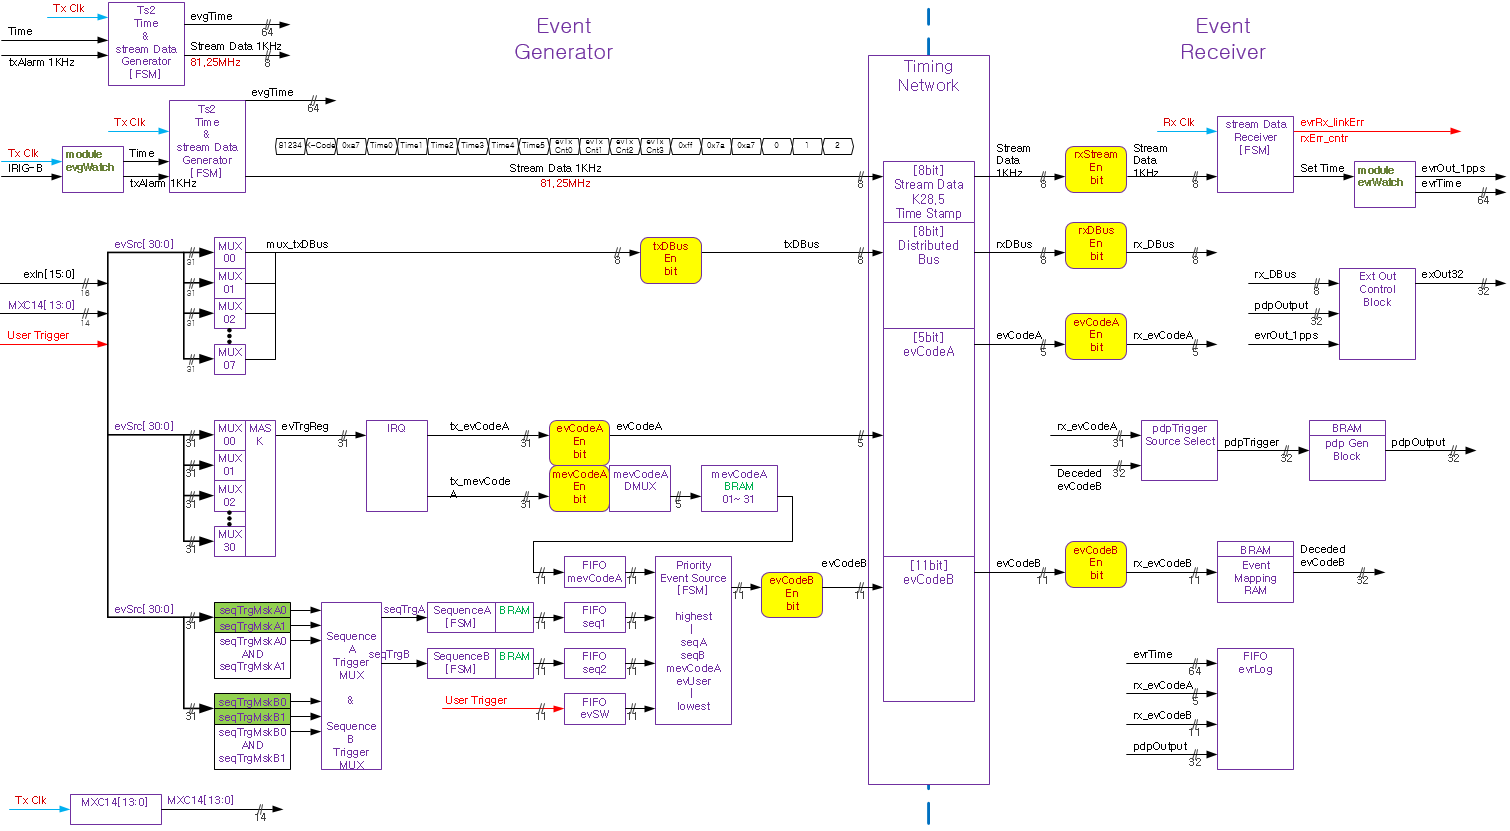
\includegraphics[width=25cm,height=10cm]{./images/img1-1.png}
\end{figure}
\begin{itemize}
	\item Xilinx Zynq XC7Z035, ARM Cortex-A8 MPCore
	\item DDR (4G)/Flash(256M) Memory, Cross Point Switch (16:16)
	\item TTL I/O (LVTTL, LVDS), SFP+ Module(1310nm LC Type)
	\item Vivado 14.6 with Xilinx SDK, Cross Compile Toolchain
\end{itemize}

\begin{figure}[H]
	\centering
	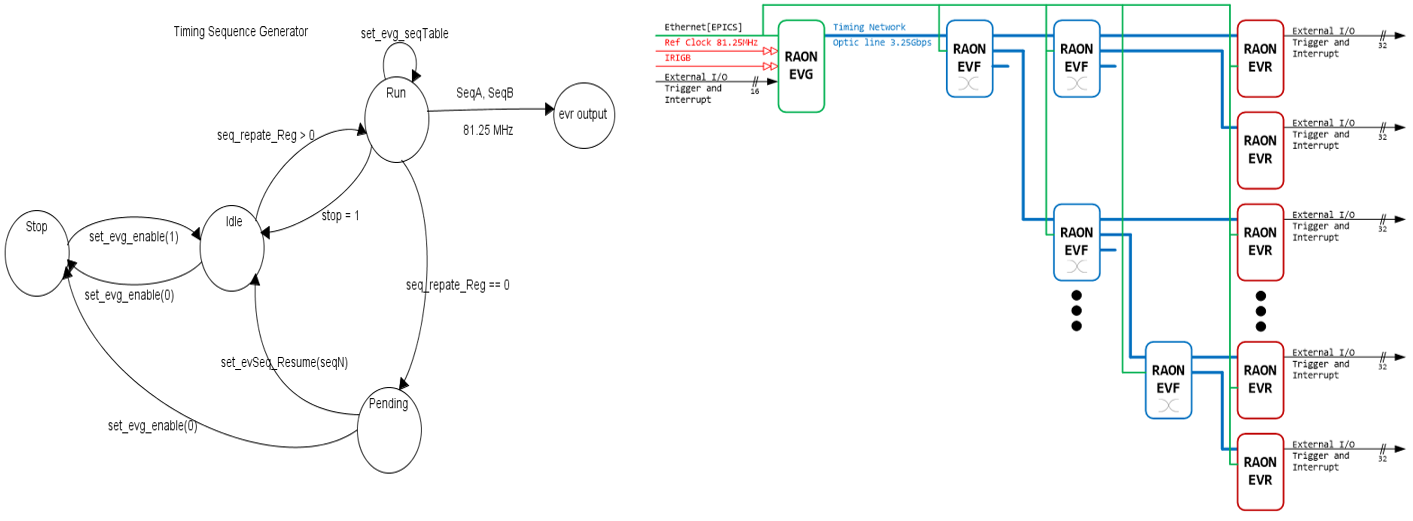
\includegraphics[width=25cm,height=10cm]{./images/dev_img_1.png}
\end{figure}
\begin{itemize}
	\item Xilinx Zynq XC7Z035, ARM Cortex-A8 MPCore
	\item DDR (4G)/Flash(256M) Memory, Cross Point Switch (16:16)
	\item TTL I/O (LVTTL, LVDS), SFP+ Module(1310nm LC Type)
	\item Vivado 14.6 with Xilinx SDK, Cross Compile Toolchain
\end{itemize}

\end{mdframed}

%\subsection*{Timing System Configruation Overview}
\vspace{2mm}
\begin{mdframed}[roundcorner=10pt]

\begin{figure}[H]
  \centering
  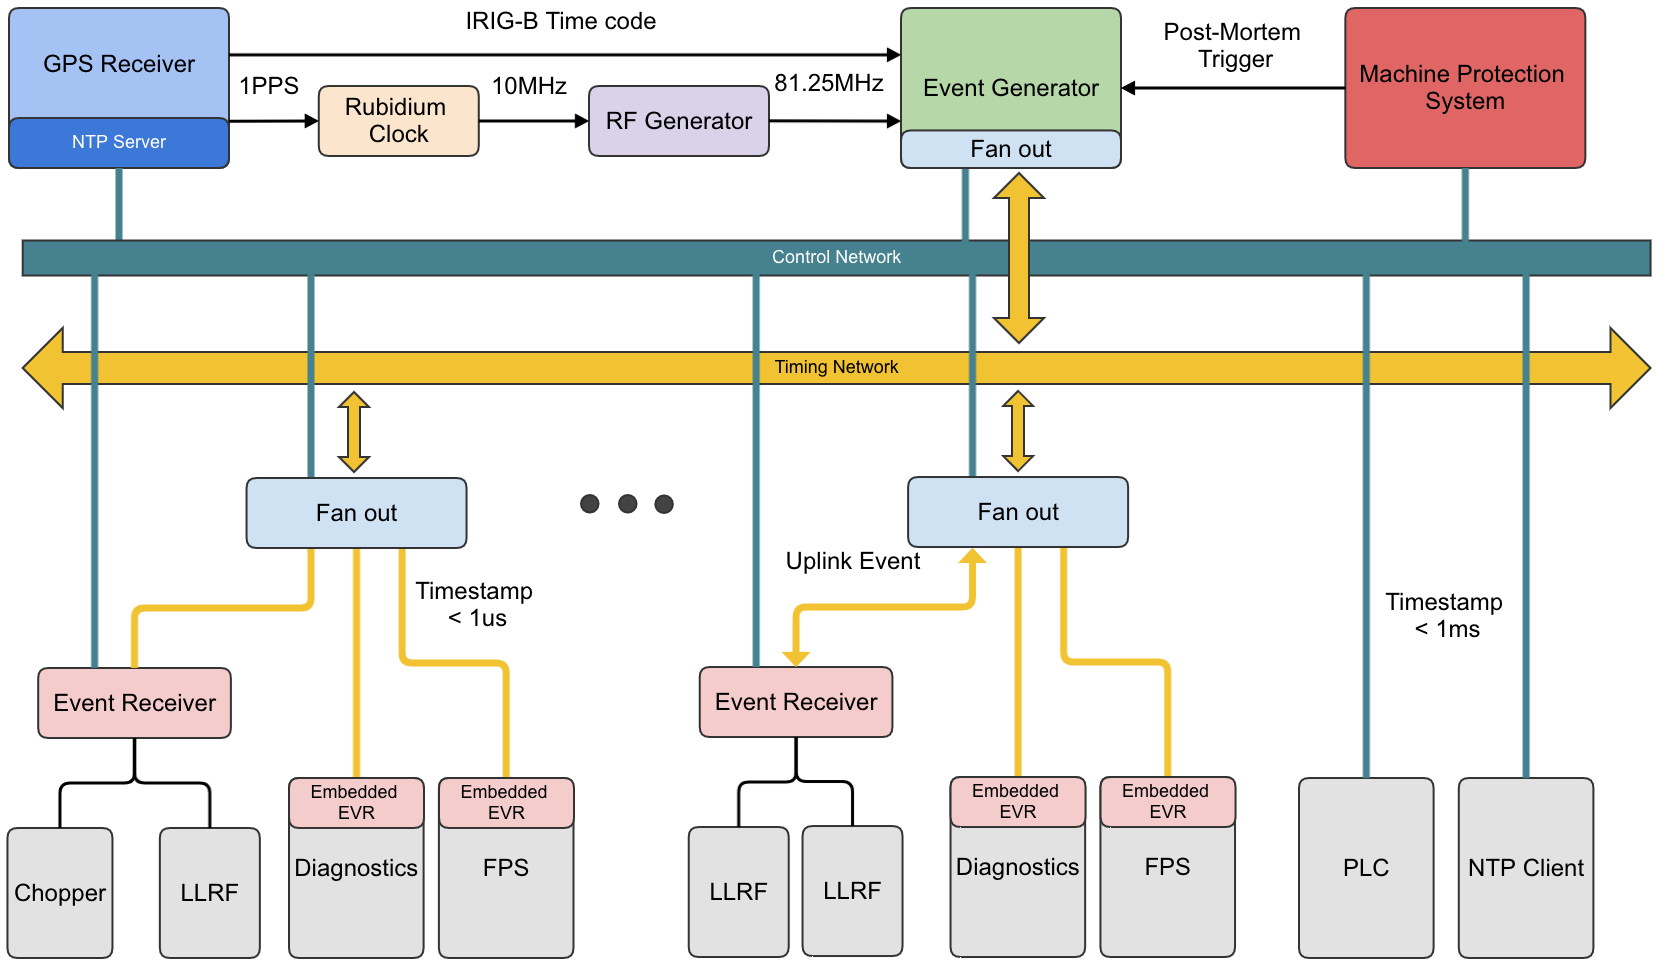
\includegraphics[width=25cm,height=12cm]{./images/raon-timing-system-scheme.png}
  \label{fig:timing_prototype}
\end{figure}
Clock signal from the RF master oscillator is synchronized with the 1PPS signal of GPS\cite{frib_timing,taiwan_timing}. The EVG module receives the RF reference clock and the 1 PPS IRIG-B signal. The timing stream data of EVG module is transmited at the optical speed of 3.25 Gbps data link (40bits * 81.25 MHz), and the time accuracy for the timestamp synchronization is less than 1 micro-second. The EVG provides the events with timestamp to Chopper, LLRF, beam diagnostics equipments, and any other devices needed the timing event\cite{frib_timing,taiwan_timing}.

\begin{figure}[H]
	\centering
	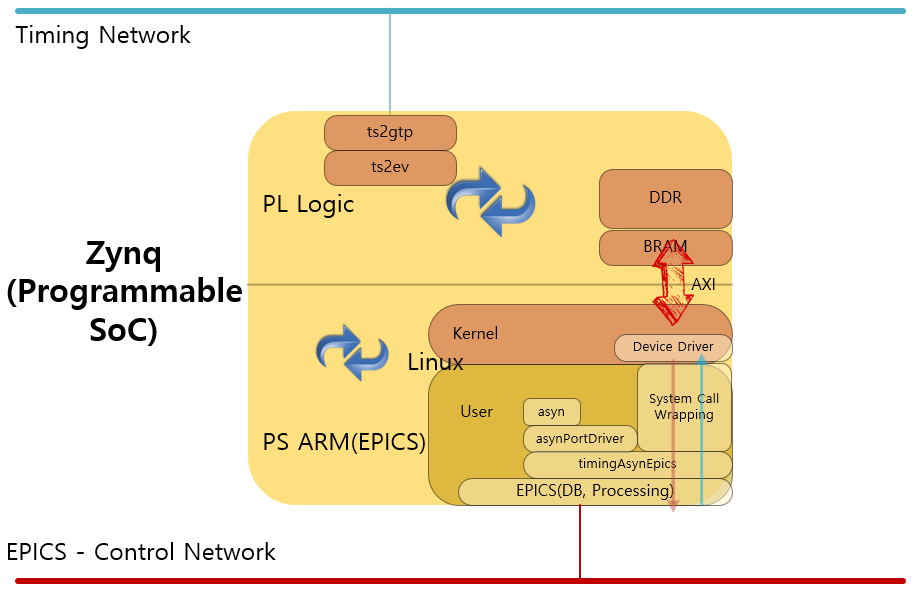
\includegraphics[width=18cm,height=8cm]{./images/img24.png}
\end{figure}

HW and SW resource needed to develop RAON timing system as follows:
\begin{itemize}
	\item Xilinx Zynq XC7Z035, ARM Cortex-A8 MPCore
	\item DDR (4G)/Flash(256M) Memory, Cross Point Switch (16:16)
	\item TTL I/O (LVTTL, LVDS), SFP+ Module(1310nm LC Type)
	\item Onboard Clock, PL(50MHz), PS(33.33MHz)
	\item Linux Kernel 4.6.0, Boot loader (U-boot)
	\item Device Driver (ts2ev, raonts2gtp)
	\item EPICS Base R3.14.15.2
	\item Asyn/AsynDriverport/timingAsynPort
	\item Vivado 14.6 with Xilinx SDK, Cross Compile Toolchain
\end{itemize}
\end{mdframed}

\section*{\centering Results}
\vspace{2mm}
\begin{mdframed}[roundcorner=10pt]

\begin{figure}[H]
	\centering
	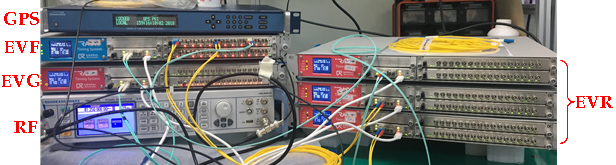
\includegraphics[width=20cm,height=5cm]{./images/img18.png}
\end{figure}
\begin{itemize}
	\item GPS Configuration and Connection to EVG decoding IRIG-B with 1PPS
	\item RF Signal Generation (81.25 MHz) to EVG
	\item EVG Connection to EVF(Fan-out) with Optical Cable
	\item EVF Fan-out to 3 EVRs with Optical Cable
	\item EVG/EVR Configuration, Verified as Follows:
\end{itemize}

\begin{figure}[H]
	\centering
	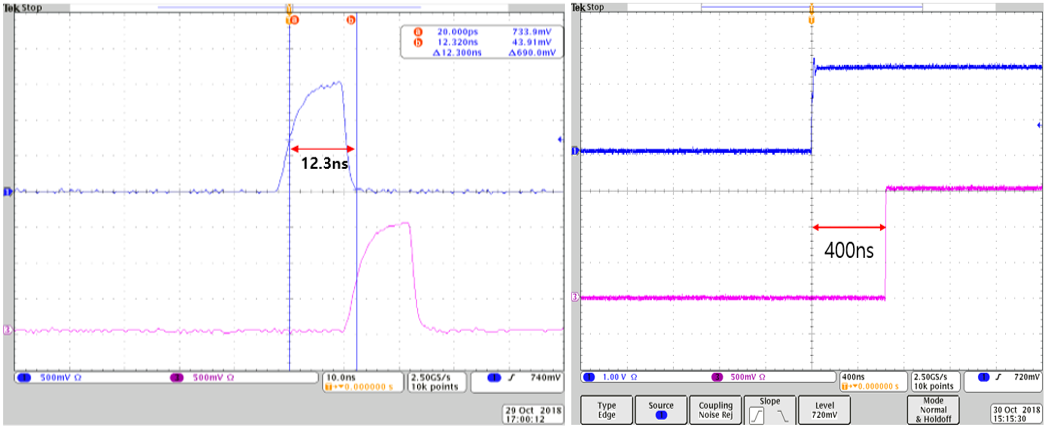
\includegraphics[width=25cm,height=8cm]{./images/result_1.png}
\end{figure}
\begin{itemize}
	\item Time Accuracy(Minimum Incremental Pulse Length) = 12.3 ns (1 clock)
	\item EVG from Post-mortem signal of FPS propagated the signal to all EVRs, the latency = 400 ns, requirment less than 1us
\end{itemize}

\begin{figure}[H]
	\centering
	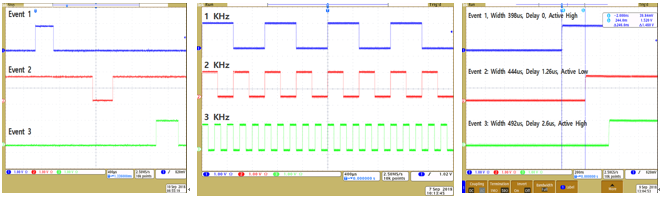
\includegraphics[width=25cm,height=8cm]{./images/result_2.png}
	\label{result_2}
\end{figure}

\begin{itemize}
	\item Event number and polarity setting from EVG, EVR output the signals as configured
	\item Using multiplexed counter of EVG, generates the various user-defined clock synchronized with RF reference clock(=81.25MHz)
	\item User-defined clock signals(1,2,3 KHz) of EVG transmitted to EVRs on the DBus
	\item Right screenshot shows that pulse width and delay time can be configurable for each signal by sequence setup
\end{itemize}

\end{mdframed}

\vspace{2mm}
\begin{mdframed}[roundcorner=10pt]

\begin{figure}[H]
	\centering
	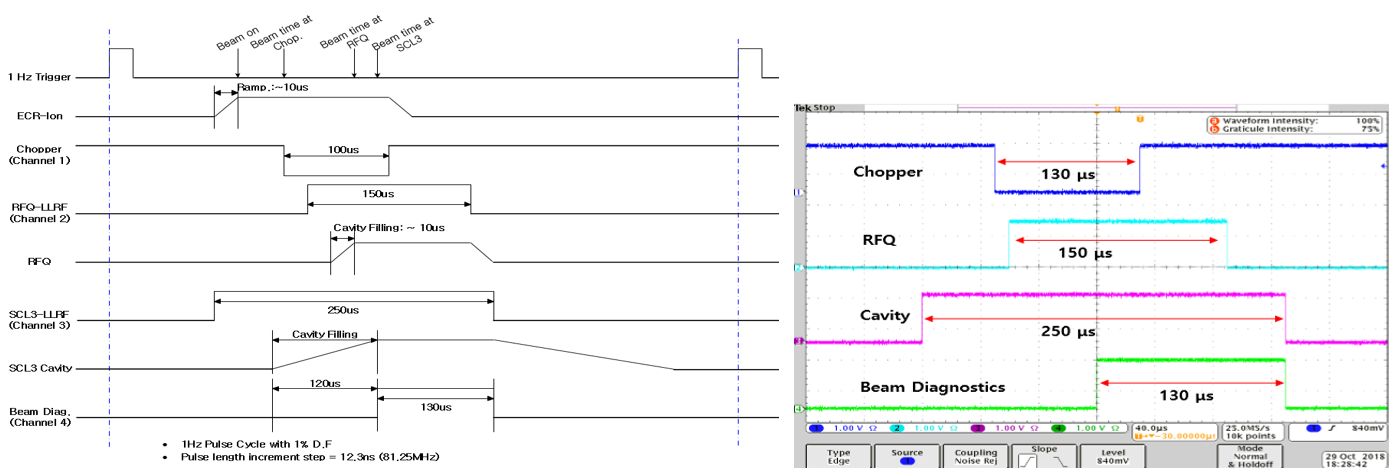
\includegraphics[width=25cm,height=15cm]{./images/result_3.png}
\end{figure}
\begin{itemize}
	\item Shows a possible timing structure scenario for SCL3 beam commissioning
	\item Repetition rate 1Hz
	\item Minimum increment pulse length 12.3ns
	\item Signals of right screen are distributed to each system according to beam commissioning scenarios.
	\item RFQ 130us pulse width with reversed polarity, RFQ 150us pulse width, Cavity at SCL3 250us pulse width, Beam Diagnostics at SCL3 130us
\end{itemize}
	
\begin{figure}[H]
	\centering
	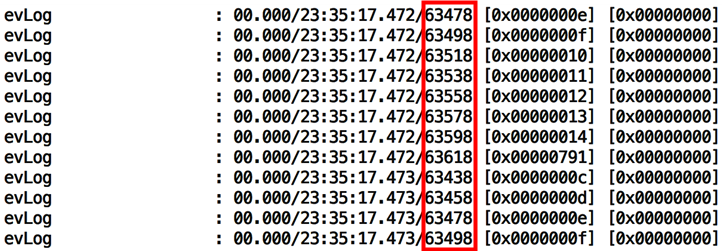
\includegraphics[width=25cm,height=6cm]{./images/result_4.png}
\end{figure}

\begin{itemize}
	\item Timestamped Event Sequence Log Test
	\item Events registered in the sequence table are sequentially transmitted as configured, 20 clocks relatively.
	\item And the timestamp of the output is normally recorded with user-defined clock(20 clock interval) as a log data like upper picture.
\end{itemize}
	
\end{mdframed}

\section*{\centering Conclusion}
\vspace{2mm}
\begin{mdframed}[roundcorner=10pt]
Timing system is one of the important control systems for the pulse operation of beam in accelerator facility.The prototye of the RAON timing system has been developed very successfully in cooperation with RISP and Korean company for one and a half year. It was improved the performance, increased the flexibility, and become a cost saving compared to existing products. As a result of the final product test, it met all the requirements of the RAON timing system (event generation and transmission synchronized to 81.25 MHz, timestamp less than 1 us,  configurable delayed pulse width, and full integration with EPICS). In the future, it will be continously applied by adding functions such as tens of ns time-stamp synchronization, and waveform for the EVR's signal verification.
\end{mdframed}

\section*{\centering Acknowledgement}
\vspace{2mm}
This work is supported by the Rare Isotope Science Project funded by Ministry of Science, ICT and Future Planning \textbf{(MSIP)} and National Research Foundation \textbf{(NRF)} of KOREA.

\begin{thebibliography}{13}   % Use for  1-9  references
%\begin{thebibliography}{99} % Use for 10-99 references

\bibitem{risp_overview}
Overview of the Rare Isotope Science Project of the Institute for Basic Science, Sunchan Jeong, New Physics: Sae Mulli, Vol. 66, No. 12, December 2016, pp. 1458~1464

\bibitem{risp} Y.~K.~Kwon, {\it et. al},``Status of Rare Isotope Science Project in Korea'',
Few-Body Syst 54, 961-966, (2013).

\bibitem{white_rabbit}
Alexander Aulin So?derqvist Niklas Claesson (2014). ?A Timing System Application using White Rabbit?. (Master thesis, Lund University), https://www.eit.lth.se/sprapport.php?uid=732

\bibitem{gis_timing}
T. Fleck.(2009) "FAIR Accelerator Control System Baseline Technical Report". GSI. Germany. Retrieved from https://www-acc.gsi.de/wiki/pub/Timing/TimingSystemDocuments/12\_Timing-System.pdf

\bibitem{epics}
EPICS website, http://www.aps.anl.gov/epics, https://wiki-ext.aps.anl.gov/epics/index.php

\bibitem{frib_timing}
M.Konnard.(2016) ? TIMING AND SYNCRONIZATION AT FRIB?. Proceedings of PCaPAC2016, Brazil. THPOPRPO10, p105-107

\bibitem{taiwan_timing}
K.H.Hu.(2011) ?RF REFERENCE DISTRIBUTION FOR THE TAIWAN PHOTON SOURCE?. Proceedings of IPAC2011, Spain. MOPO040, p571-573

\bibitem{parallel}
S.Lee, et. a1.?Distributed and parallel real-time control system equipped FPGA-Zynq and EPICS middleware?, Proceedings of the 20th IEEE-NPSS Real Time Conference, June, 2016 


\end{thebibliography}
\end{multicols}

%\vspace{13mm}

%\begin{minipage}[b]{1\linewidth}

%\section*{RAON Major Operations Modes}
%\vspace{2mm}
%\begin{figure}[H]
 % \includegraphics[width=0.99\columnwidth]{./images/raon_all_modes.eps}
%\end{figure}

%\end{minipage}

\end{document}

